\documentclass[11pt, a4paper]{article}
%\usepackage{proj1}
\usepackage{natbib}
\usepackage{fancyhdr}  
\usepackage{subcaption}
\usepackage{caption}
\usepackage{graphicx}
\usepackage{numprint}
\usepackage{multirow}
\linespread{1.25} 
\setlength{\parindent}{0cm}
\graphicspath{{Images/}}
\usepackage{hyperref}
\usepackage{amsmath}
\usepackage{amsfonts}
\usepackage{amssymb}
\usepackage{amsthm}
\usepackage{mathtools}
\usepackage{commath}
\usepackage{bbm}

%\usepackage[sc,osf]{mathpazo}
\usepackage{subcaption}
\usepackage[a4paper, top=1in, left=1.0in, right=1.0in, bottom=1in, includehead, includefoot]{geometry} %Usually have top as 1in

\usepackage{listings}
\usepackage{color} %red, green, blue, yellow, cyan, magenta, black, white
\definecolor{mygreen}{RGB}{28,172,0} % color values Red, Green, Blue
\definecolor{mylilas}{RGB}{170,55,241}


\hypersetup{colorlinks,linkcolor={black},citecolor={blue},urlcolor={black}}
\usepackage{color}
\urlstyle{same}


\theoremstyle{definition}
\newtheorem{definition}{Definition}[section]

\newcommand{\adja}{q_a}
\newcommand{\adjb}{q_b}
\newcommand{\adjaB}{q_{a,\partial \Omega}}
\newcommand{\adjbB}{q_{b,\partial \Omega}}
\newcommand{\adjB}{q_{\partial \Omega}}
\newcommand{\Adja}{\mathbf{p}}
\newcommand{\Adjb}{q}
\newcommand{\adj}{q}
\newcommand{\Adjc}{{q}_{\partial \Omega}}
\newcommand{\ra}{\rho_a}
\newcommand{\rb}{\rho_b}
\newcommand{\w}{\mathbf{w}}
\newcommand{\f}{\mathbf{f}}
\newcommand{\ve}{\mathbf{v}}
\newcommand{\n}{\mathbf{n}}
\newcommand{\h}{\mathbf{h}}
\newcommand{\K}{\mathbf{K}}
\newcommand{\hr}{\widehat \rho}

%	\begin{figure}[h]
%		\centering
%		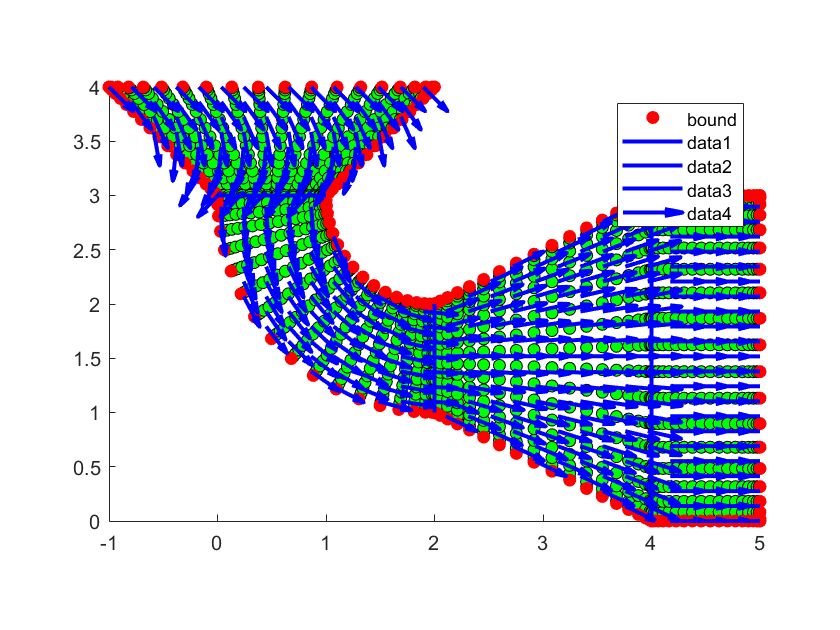
\includegraphics[scale=0.35]{F1.png}
%		\caption{Forward $\rho$ for $a = 0.01$} 
%		\label{F1}
%	\end{figure}

\begin{document}
	\section*{Time independent flow control}
	\section{Deriving the Gradient Equation}
	We have the following OCP:
	\begin{align*}
		&J = \frac{1}{2}\int_0^T \int_\Omega (\rho - \widehat \rho)^2 dr dt + \frac{\beta}{2} \int_\Omega \w(r)^2 dr\\
		&\text{subject to:}\\
		&\frac{\partial \rho}{\partial t} = \nabla^2 \rho - \nabla \cdot (\rho \w(r))
	\end{align*}
Note however, that the following result can be found with any other forward problem. Since the derivative of the Lagrangian with respect to $\w$ is taken, any terms that do not involve $\w$ can be exchanged without changing the resulting gradient equation.
	The Lagrangian is:
	\begin{align*}
		\mathcal{L}(\rho,\w, q) &=  \frac{1}{2}\int_0^T \int_\Omega (\rho - \widehat \rho)^2 dr dt + \frac{\beta}{2} \int_\Omega \w(r)^2 dr \\
		&- \int_0^T \int_\Omega q\frac{\partial \rho}{\partial t} - q\nabla^2 \rho + q\nabla \cdot (\rho \w) dr dt.
	\end{align*}
	And after integrating by parts (neglecting the BCs because they are unchanged from before):
	\begin{align*}
		\mathcal{L}(\rho,\w, q) &=  \frac{1}{2}\int_0^T \int_\Omega (\rho - \widehat \rho)^2 dr dt + \frac{\beta}{2} \int_\Omega \w(r)^2 dr \\
		&- \int_0^T \int_\Omega q\frac{\partial \rho}{\partial t} - q\nabla^2 \rho -  \rho \w \cdot \nabla q dr dt.
	\end{align*}
	Taking derivatives with respect to $\w$ gives:
	\begin{align*}
		\mathcal{L}_\w(\rho,\w, q)h &= \int_\Omega \beta \w(r) \cdot \h(r) dt + \int_0^T \int_\Omega \rho \h(r) \cdot \nabla q dr dt.
	\end{align*}
	Since $\w$ does not depend on $t$, neither does $\h$ and so this can be taken out of the time integral:
	\begin{align*}
		\mathcal{L}_\w(\rho,\w, q)h &= \int_\Omega \bigg( \beta \w(r) \cdot \h(r)  + \h(r) \cdot \int_0^T \rho  \nabla q dt \bigg) dr.
	\end{align*}
	Then we get:
	\begin{align*}
		\beta \w(r)  +  \int_0^T \rho  \nabla q dt = 0
	\end{align*}
	And finally:
	\begin{align*}
		\w(r) = - \frac{1}{\beta} \int_0^T \rho  \nabla q dt
	\end{align*}
	\section{Numerical Application to the Sedimentation Equation}
	This result can be used for other forward problems as well, since only the terms involving the control are affected here. Therefore, we apply the result to the sedimentation equations.
	We have $N = 40$ and $n = 30$ for each shape. We choose the ODE tolerance to be $10^{-7}$ and the optimization tolerance is $10^{-3}$.
	I set up a test problem which sets $\hr$ to be the forward solution for $V_{ext} = ay$, where $a = 0.1$, as in Archer's paper. Then I set up the optimization forward problem to be such that $a = 0.01$ and $\w = \mathbf 0$. We expect the control to act downward, since the strength of gravity $a$ is decreased.
	We also expect that the cost $\mathcal J$ is decreasing from the baseline $J_{FW}$ when optimizing.
	The gradient equation is:
	\begin{align*}
		\w = - \frac{1}{\beta}\int_0^T \rho \nabla q dt.
	\end{align*}
	This means, we get a $\w$ which is averaged over the time horizon and therefore time independent. This seems to work well. $J_{FW} = 0.4855$ and $J_{Opt} = 0.0733$. The results can be seen in Figures \ref{F6}, \ref{F7} and \ref{F8}.
	
	\begin{figure}[h]
		\centering
		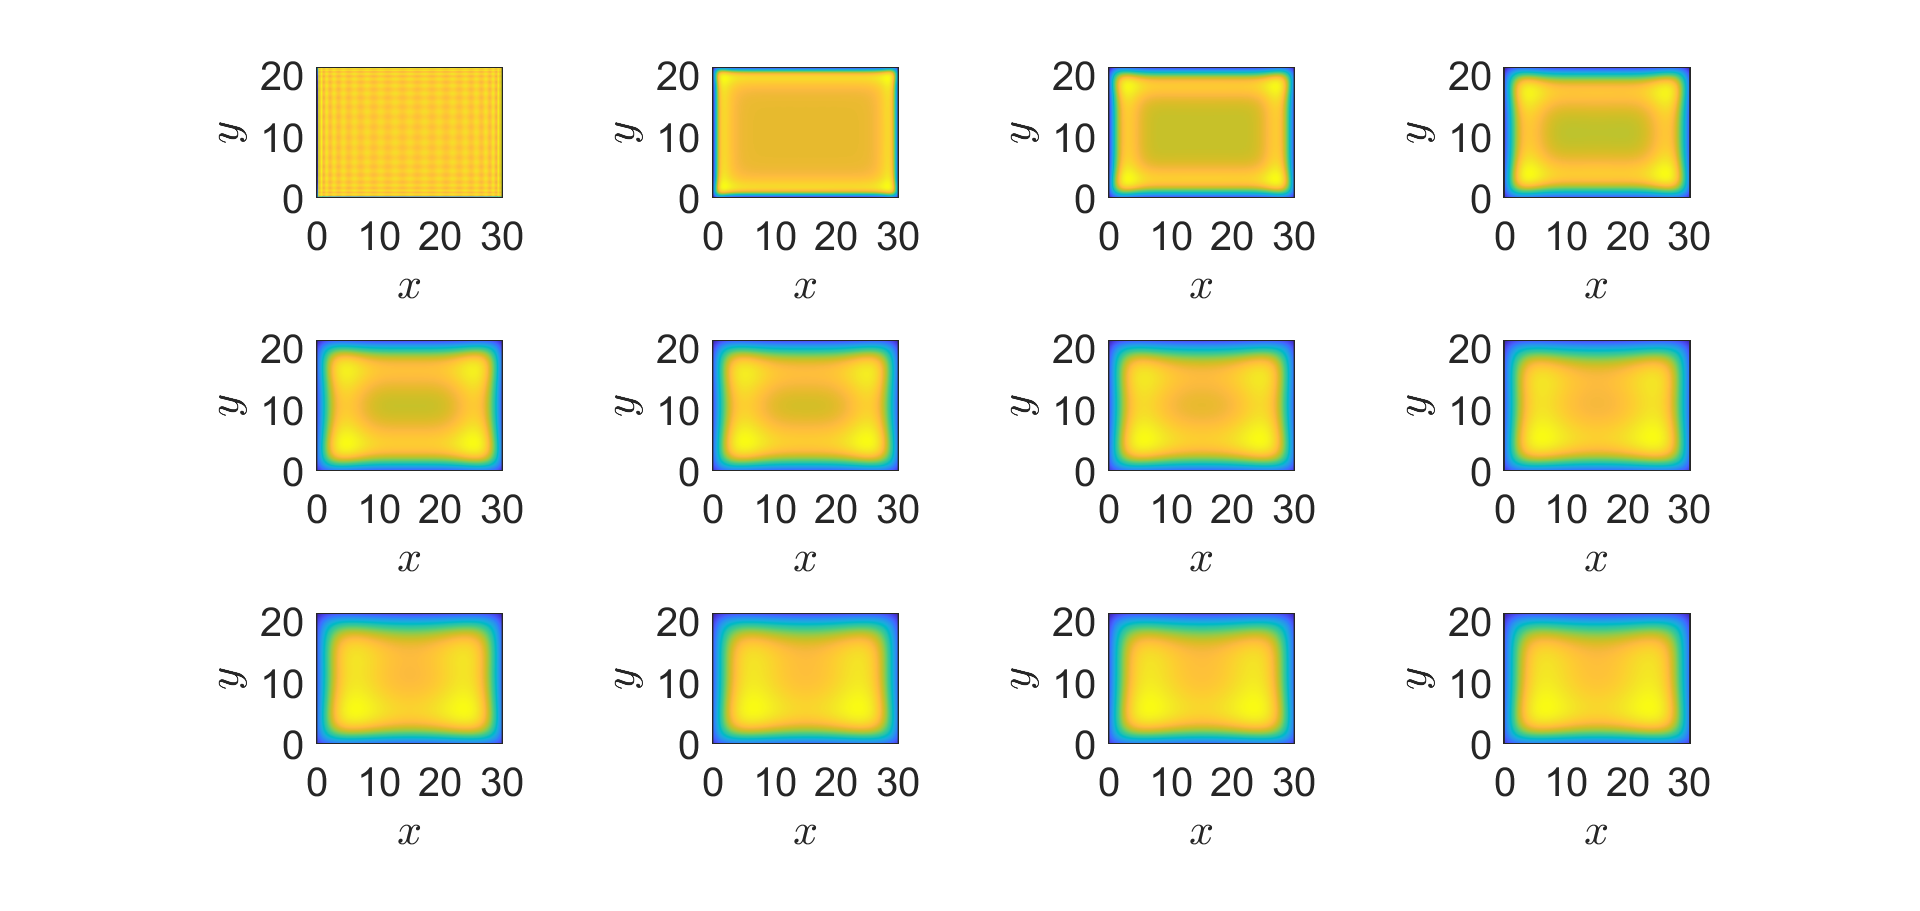
\includegraphics[scale=0.35]{C1.png}
		\caption{Time-independent; Forward $\rho$ for $a = 0.01$} 
		\label{F6}
	\end{figure}	
	\begin{figure}[h]
		\centering
		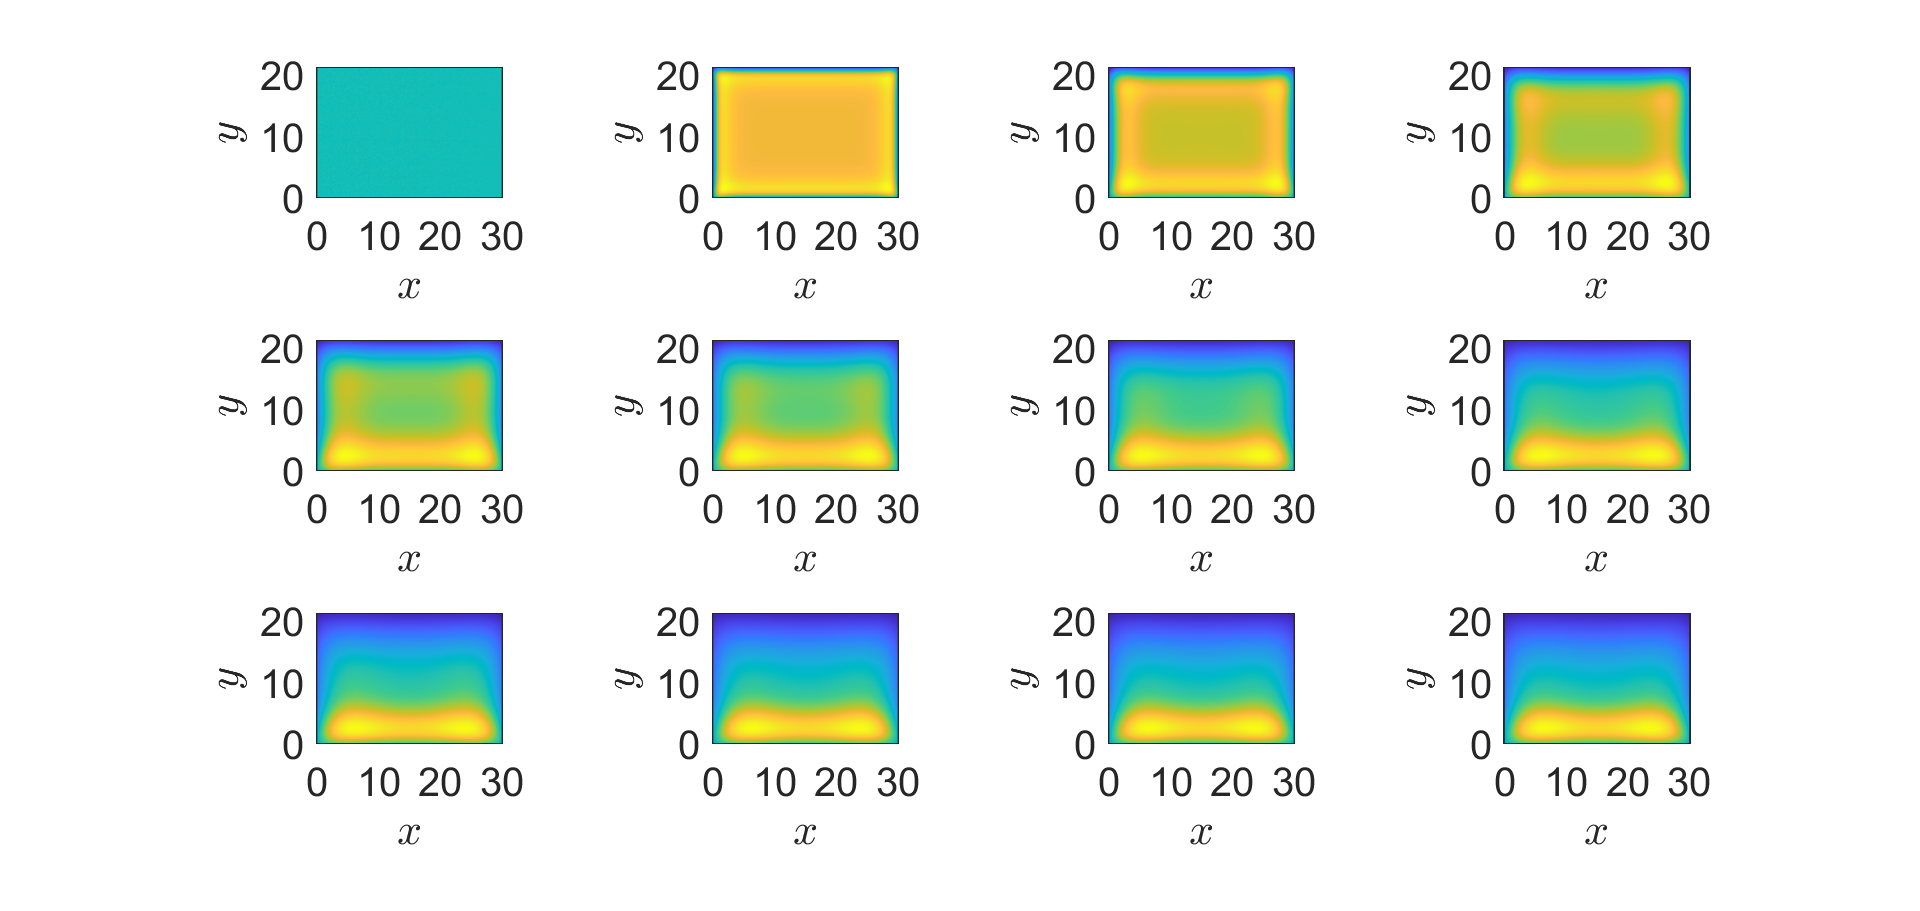
\includegraphics[scale=0.35]{C2.png}
		\caption{Time-independent; Optimal $\rho$ for $a = 0.01$} 
		\label{F7}
	\end{figure}
	\begin{figure}[h]
		\centering
		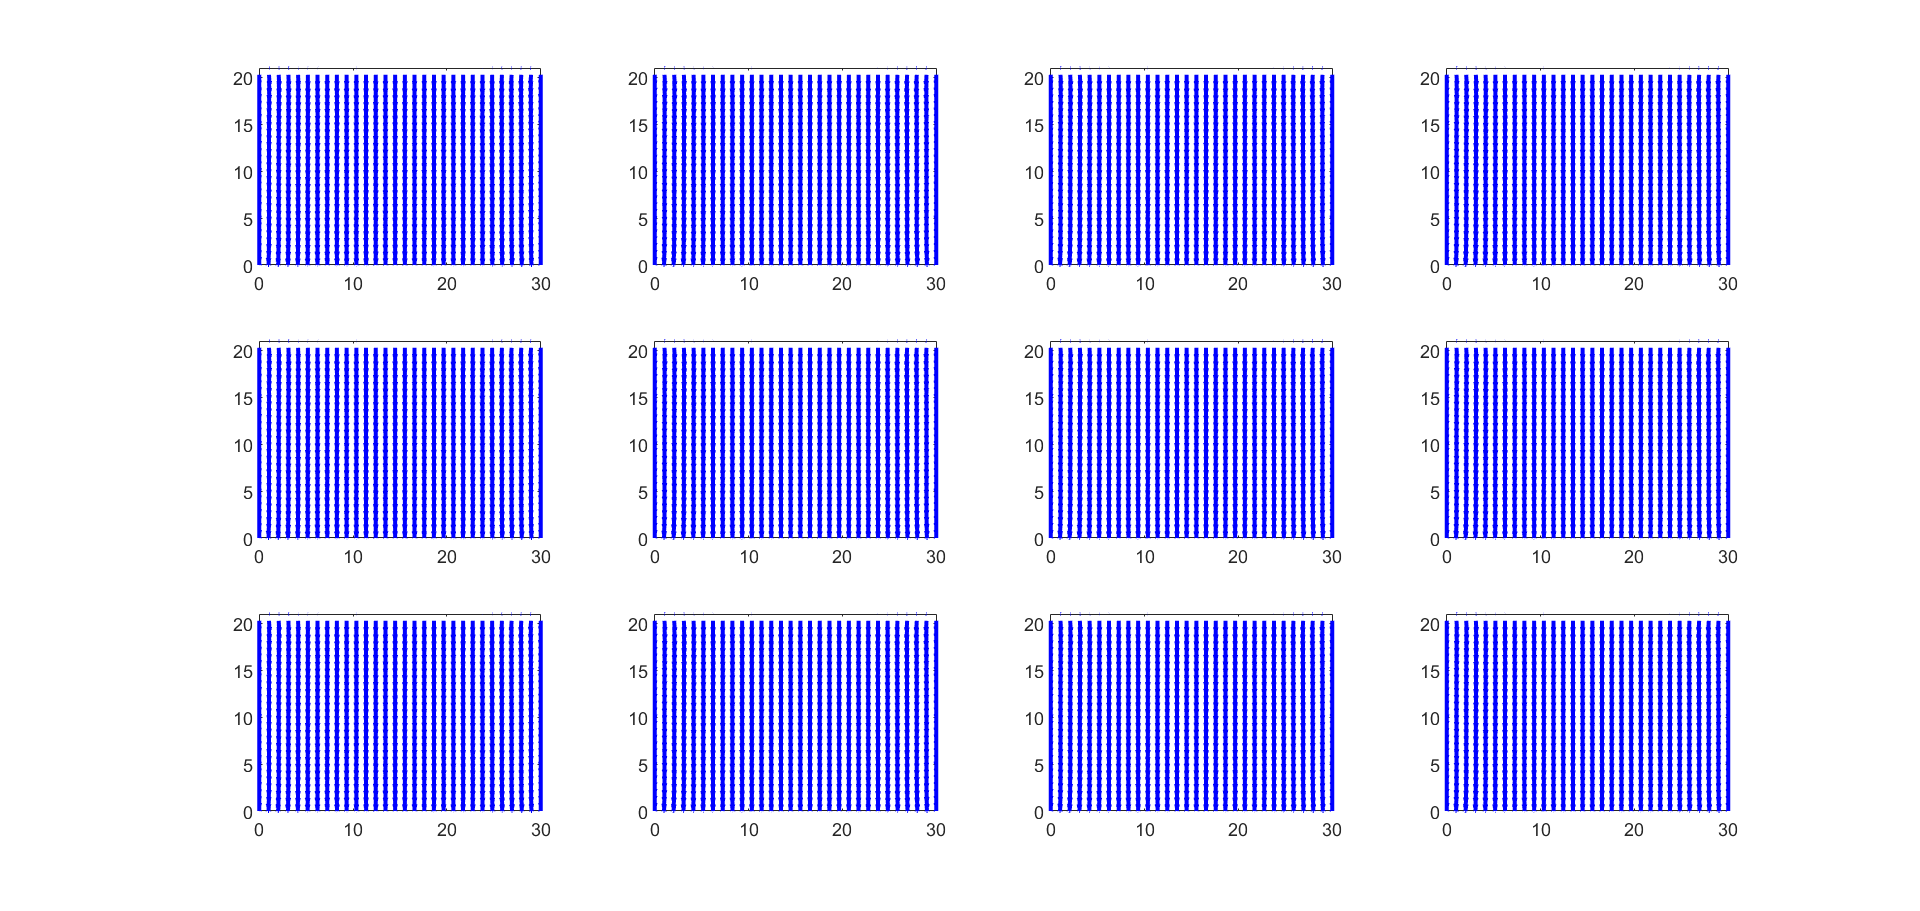
\includegraphics[scale=0.35]{C3.png}
		\caption{Time-independent; Optimal Control for $a = 0.01$} 
		\label{F8}
	\end{figure}
	
	
	
	
	
	\subsection{Comparison of control to original $V_{ext}$}
	We wanted to see whether the time independent flow control is similar to the $\nabla V_{ext}$ of the target.
	The target state was influenced by $V_{ext} = 0.1 y_2$. The forward state for the OCP was influenced by $V_{ext} = 0.01 y_2$. 
	Figure \ref{F1} shows the control and $\nabla V_{ext}$ of the target. We can see that one of these is positive, while the other one is negative. This is due to the opposite signs of $\w$ and $\nabla V_{ext}$ in the PDE.
	
	\begin{figure}[h]
		\centering
		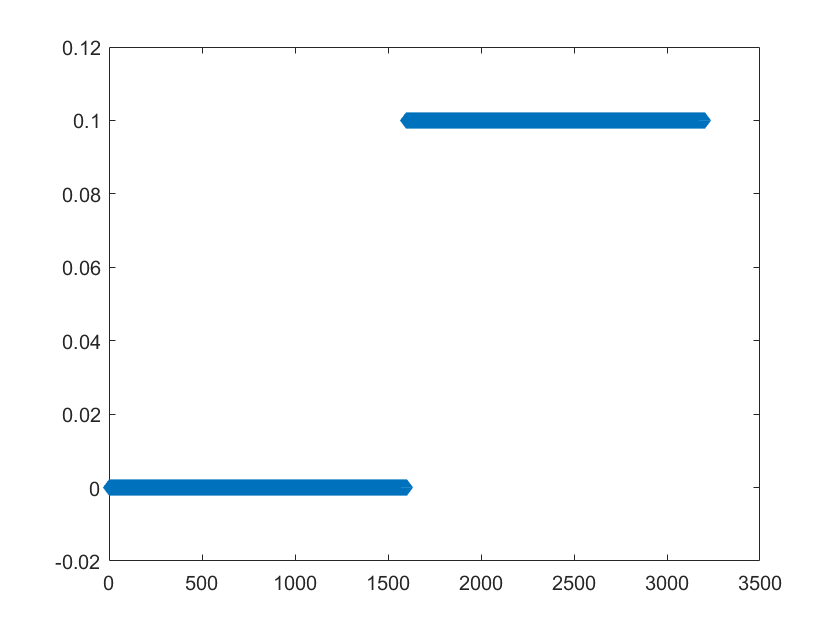
\includegraphics[scale=0.35]{V1.png}
		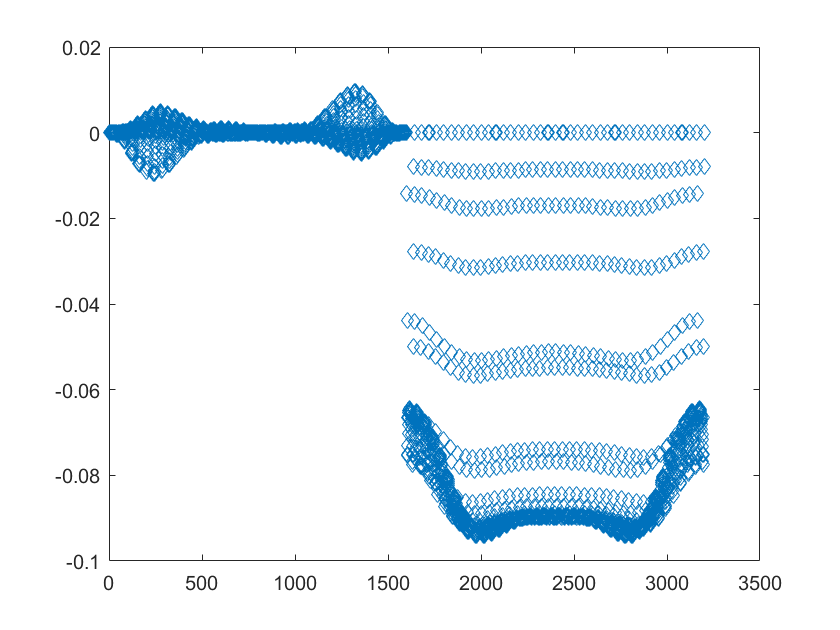
\includegraphics[scale=0.35]{W1.png}
		\caption{$\nabla V_{ext}$ of target and optimal control $\w$.} 
		\label{F1}
	\end{figure}
	
\end{document}